
\begin{definition}
Una función es \textbf{periódica} de período $p$ si, para todo valor de $x$ perteneciente al dominio de la función, se verifica que $f(x+p)=f(x)$.
\end{definition}
\geogebra{bqzcquyw}
Si una función es periódica de período $p$, sus valores y, por tanto, su gráfica, se repiten en intervalos sucesivos de amplitud $p$.\\
Las funciones periódicas se estudian en un intervalo de amplitud $p$, y para construir el resto de la gráfica, solamente debemos de trasladar dicho estudio al resto del dominio de la función.
\youtube{dTgrxlz6bMs}
\subsubsection{Ejercicios}

\begin{scq}
	Selecciona la opción correcta:\\
	\begin{figure}
		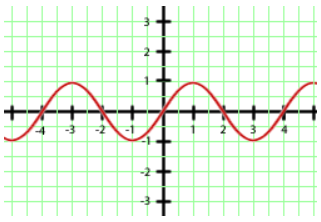
\includegraphics{samples/propiedades/periodicidad1.jpg}
	\end{figure}
	\begin{choices}
		\begin{choice}
			La función es periódica con periodo $T=2$.	
		\end{choice}
		\begin{choice}[x]
			La función es periódica con periodo $T=4$.
		\end{choice}	
		\begin{choice}
			La función no es periódica.
		\end{choice}
	\end{choices}
	\begin{feedback}
		Sus imágenes se repiten periódicamente en intervalos de longitud 4, por lo que la función es periódica con periodo $T=4$.
	\end{feedback}
\end{scq}

\vspace{1cm}


\begin{scq}
	Selecciona la opción correcta:\\
	\begin{figure}
		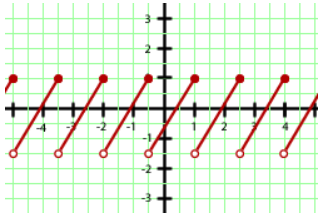
\includegraphics{samples/propiedades/periodicidad2.jpg}
	\end{figure}
	\begin{choices}
		\begin{choice}[x]s
			La función es periódica con periodo $T=2$.	
		\end{choice}
		\begin{choice}
			La función es periódica con periodo $T=4$.
		\end{choice}	
		\begin{choice}
			Ninguna de las respuestas anteriores es correcta.
		\end{choice}
	\end{choices}
	\begin{feedback}
		Sus imágenes se repiten periódicamente en intervalos de longitud 4, por lo que la función es periódica con periodo $T=2$.
	\end{feedback}
\end{scq}

\vspace{1cm}


\begin{scq}
	Selecciona la opción correcta:\\
	\begin{figure}
		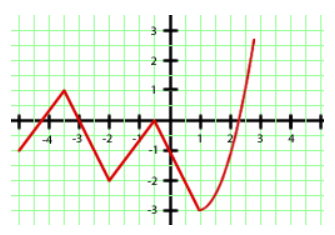
\includegraphics{samples/propiedades/periodicidad3.jpg}
	\end{figure}
	\begin{choices}
		\begin{choice}
			La función es periódica con periodo $T=5$.	
		\end{choice}
		\begin{choice}
			La función es periódica con periodo $T=6$.
		\end{choice}	
		\begin{choice}[x]
			La función no es periódica.
		\end{choice}
	\end{choices}
	\begin{feedback}
		No hay intervalos de igual longitud donde se repiten las imágenes, por lo que la función no es periódica.
	\end{feedback}
\end{scq}



\begin{scq}
	Selecciona la opción correcta:\\
	\begin{figure}
		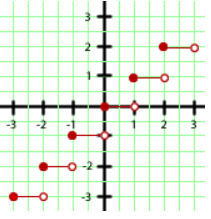
\includegraphics{samples/propiedades/periodicidad4.jpg}
	\end{figure}
	\begin{choices}
		\begin{choice}
			La función es periódica con periodo $T=1$.	
		\end{choice}
		\begin{choice}[x]
			La función es periódica con periodo $T=2$.
		\end{choice}	
		\begin{choice}[x]
			La función no es periódica.
		\end{choice}
	\end{choices}
	\begin{feedback}
		No hay intervalos de igual longitud donde se repiten las imágenes, por lo que la función no es periódica.
	\end{feedback}
\end{scq}



\begin{scq}
	Selecciona la opción correcta:\\
	\begin{figure}
		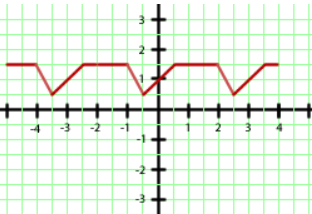
\includegraphics{samples/propiedades/periodicidad5.jpg}
	\end{figure}
	\begin{choices}
		\begin{choice}
			La función es periódica con periodo $T=-3$.	
		\end{choice}
		\begin{choice}[x]
			La función es periódica con periodo $T=3$.
		\end{choice}	
		\begin{choice}
			La función no es periódica.
		\end{choice}
	\end{choices}
	\begin{feedback}
		Sus imágenes se repiten periódicamente en intervalos de longitud 3, por lo que la función es periódica con periodo $T=3$.
	\end{feedback}
\end{scq}
